\documentclass[11pt,letterpaper,landscape]{article}
\usepackage[utf8]{inputenc}
\usepackage[T1]{fontenc}
\usepackage{lmodern}
\usepackage[letterpaper,landscape,top=1.2cm,bottom=1.2cm,left=1.2cm,right=1.2cm]{geometry}
\usepackage{graphicx}
\usepackage{tabularx}
\usepackage{amsmath}
\usepackage{booktabs}
\usepackage{xcolor}

\definecolor{navyblue}{RGB}{26, 79, 124}
\pagestyle{empty}

\begin{document}

\begin{center}
\vspace*{-0.5cm}
{\color{navyblue}\hrule height 1.5pt}
\vspace{0.15cm}
{\Large \textbf{\color{navyblue} SOLVANTA ENGINEERING SOLUTIONS S.A. DE C.V.}} \quad -- \quad
{\large \textbf{DIAGRAMA DE FLUJO DE PROCESO PRELIMINAR (PFD v0)}} \\
{\small Planta de Producción de e-Metanol ($30\,000\text{ t/año}$) a partir de $\text{CO}_2$ Capturado e Hidrógeno Electrolítico SOEC}
\vspace{0.15cm}
{\color{navyblue}\hrule height 1.5pt}

\vspace{0.1cm}
\fbox{
    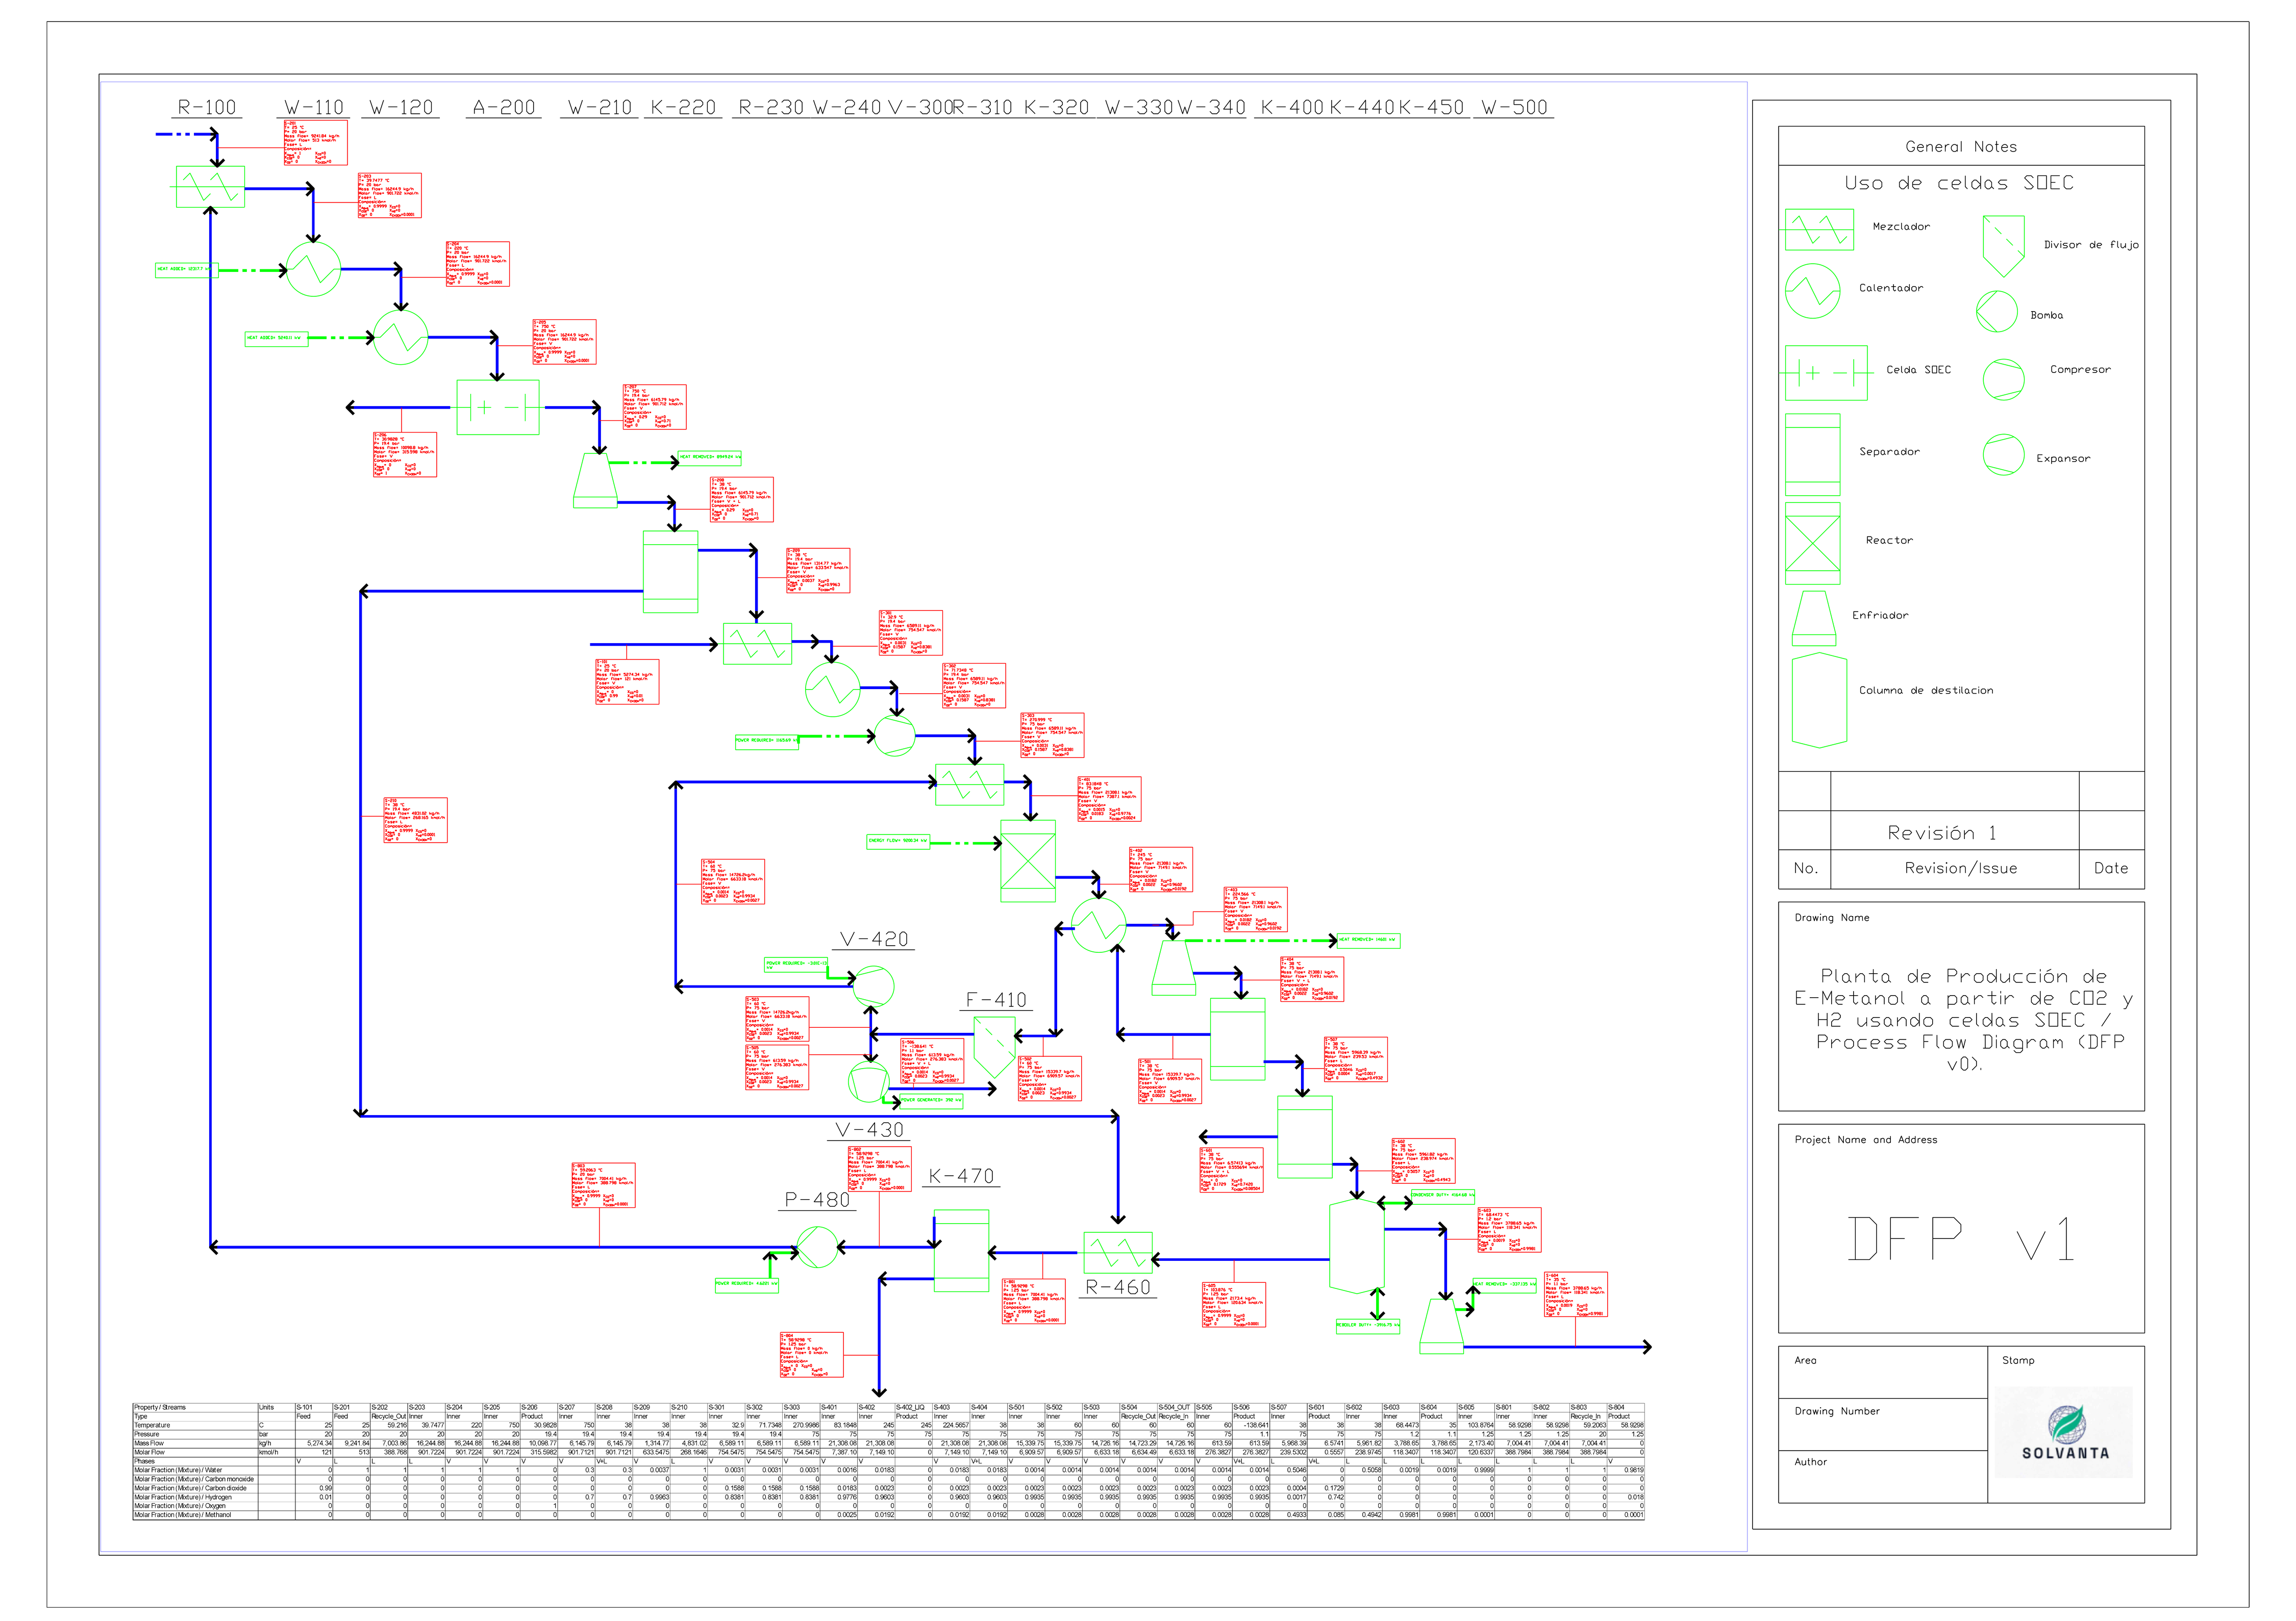
\includegraphics[width=0.96\textwidth,height=12.0cm,keepaspectratio]{dfp_plpl_1_1.png}
}

\vspace{0.15cm}
\footnotesize
\begin{tabularx}{0.98\textwidth}{|p{4.5cm}|X|c|p{4.5cm}|}
\hline
\textbf{PROYECTO:} & \textbf{NOTAS GENERALES DE DISEÑO:} & \textbf{REV:} & \textbf{APROBACIÓN TÉCNICA:} \\
Planta de e-Metanol $30\,\text{kt/año}$ & 1. Base de operación: 8\,000 h/año en régimen continuo ($3\,750.0\text{ kg/h}$ netos). & v0.2 & \textbf{Solvanta Engineering Solutions} \\
Lic.: RFP-CCM-EM-001 & 2. Paquete SOEC EL-201 opera a $750^\circ\text{C}$ con vapor saturado (Área 200). & & Ing. Karol Paola Camacho López \\
Doc: PFD-v0\_Solvanta.pdf & 3. Síntesis catalítica en reactor multitubular BWR R-401 a $75\text{ bar}, 245^\circ\text{C}$ (Área 400). & & Fecha: 14 de septiembre de 2026 \\
Caso DWSIM: Aprobado & 4. Purga continua de $4\%$ a turboexpansor X-501 ($390.43\text{ kW}$ recuperados). & & Estandarización de corrientes: \\
Nomenclatura: S-101 a S-804 & 5. Nomenclatura normalizada: S-101 a S-804 por áreas de proceso (100-800). & & Áreas 100, 200, 300, 400, 500, 600, 800 \\
\hline
\end{tabularx}
\end{center}

\end{document}